\newpage
\usecasebase{Inserimento di \textit{feedback}}
\label{usecase:Inserimento di feedback}

\begin{figure}[h]
	\centering
	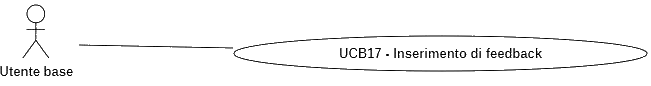
\includegraphics[width=0.8\textwidth]{./uml/UCB17.png} 
	\caption{Inserimento di \textit{feedback}}
	\label{fig:UCB16}
  \end{figure}

\begin{itemize}
	\item \textbf{Attore principale:} Utente base.

	\item \textbf{Precondizione:} L'Utente base ha completato un ordine che si
	      trova nello stato "Terminato".

	\item \textbf{Postcondizione:} L'Utente base ha lasciato un \textit{feedback}.

	\item \textbf{Scenario principale:}
	      \begin{enumerate}
		      \item L'Utente base seleziona la prenotazione per la quale vuole
		            lasciare un \textit{feedback} (vedi
		            \autoref{usecase:Visualizzazione del riepilogo prenotazione});

		      \item L'Utente base compila il \textit{form} del \textit{feedback} del ristorante;

		      \item L'Utente base conferma il \textit{feedback};

		      \item Il Sistema registra il \textit{feedback};

		      \item Il Sistema aggiorna la media dei punteggi del ristorante.

	      \end{enumerate}
\end{itemize}
